\documentclass{./llncs2e/llncs}
\usepackage{graphicx}

\usepackage{float}
%\usepackage{mathtools}
\usepackage[utf8]{inputenc}
\usepackage[nolist,nohyperlinks]{acronym}
% Maintain images and tables within their respective sections
\usepackage[section]{placeins}
\graphicspath{{img/}}

\usepackage{authblk}
\usepackage[pdfborder={0 0 0}]{hyperref}% For email addresses
%
% Change the margins
%
% \usepackage[margin=2.9cm]{geometry}
\author{Filipe Apolinário, João Rocheteau, and Gil Dias}
\institute{Instituto Superior Técnico}

\begin{document}
\title{DynamysisPHP Tool}
\subtitle{A tool for providing dynamic analysis of common PHP attacks}

\maketitle
\section{DynamysisPHP Tool}

The DynamysisPHP Tool is a simple tool that detects common attacks against PHP code through dynamically analyzes, pinpointing where the attacked occurred (entry-point) and what sensitive elements of the system (sensitive sinks) where affected by the attack and suggesting possible ways disable the attack (sanitization functions). 

\subsection{Design Structure}
This tool is divided into two components, the parser and the analyzer tool.

When a user wants to execute a PHP program and analyze it with the DynamysisPHP Tool, the user needs to gather traces using Xdebug tool in order to gather the semantical information of the code execution. However gathering this data is not enough it needs to be normalized in order to provide meaningful information for the analyses to be effective and reduce the number of errors. Thus, before analysing the PHP program clients need to use the parser component and obtain their parsed traces and source code. Finally, the client can use the analyser in order to detect vulnerabilities on the source code.

\subsection{Parser}
The preliminary parser component is composed of two scripts, one for parsing the source code $src.sh$ and the other for parsing traces $tracer.sh$.

Regarding the source code script $src.sh$, the code written in PHP can have fail-points for analyzer component that need to be corrected in order to reduce error detection. First, the file can be have unnecessary spaces, tabulations, or blank lines that may hinder the mapping between the Xdebug trace and the source code and therefore needs to be discarded in order to improve readability for the analyzer component. Secondly, PHP allows to convert variables into strings by escaping them, e.g. the variable $\$var$ with value $8$ can be converted into a string by $"\$var"$ being replace to $"8"$. This hinders the DynamysisPHP tool quite a lot because it interprets the converted variables as a simple string and thus loosing context and missing possible vulnerabilities. Therefore, escaped string are removed and alongside with the concatenated text, replacing it to the variable in question. For example, "SELECT * FROM X WHERE $\$var$" is replaced to $\$var$. Thus providing context to the DynamysisPHP Tool without loosing any needed information. 

Regarding the tracer script $tracer.sh$, the trace given from the Xdebug is not easy to integrate with DynamysisPHP Tool and therefore needs to be parsed. In order to avoid fail-points the Xdebug traces are normalized into two types of lines: the function call lines and expression lines. Both start by an arrow ($->$ in case of function call and $=>$ in case of expression) and followed by the mapping of the line in the source code.

\subsection{Analyzer}  
The analyzer is the core component of this tool. With it, users can dynamically analyze their code and detect whether it is sensitive to common PHP vulnerabilities. This is fully provided by the analyzer by automatically tracking each information flow initiated on the source code's entry-points to the sensitive sinks and verifying if it reached them un-sanitized. If so a vulnerability was detected. To do so, alongside with the parsed trace and sourced code provided by the user, the analyzer relies on a configuration file $config.in$ that has a set of patterns of PHP common attacks including the entry points commonly used for the attack, the end-points that are affected and the sanitization functions used for neutralizing the vulnerability.

The general behaviour of this component is as follows. First the client provide the parsed source file and parsed trace file to the analyzer. Then, $config.in$ file is loaded and the user provided files are tested against each vulnerability present on the $config.in$ file. To do so, for each vulnerability a new system state is generated where each information-flow is tracked from the entry-point to each sensitive-sink. Gathering states of the variables assigned to the un-sanitized entry-points values (marking them as 'tainted') and updating their state to 'untainted' as they pass along sanitization functions. Whenever a tainted variable reaches the sensitive-sink the program is vulnerable to the vulnerability being tested. The two possible scenarios for the analyzer, where a variable is sanitized and reaches the sink (no vulnerability present) and where the unsanitized variable reaches the sink (vulnerability present), can be seen respectively in figures \ref{fig:right} and \ref{fig:wrong}.

\begin{figure}
	\centering
	\begin{minipage}{.5\textwidth}
		\centering
		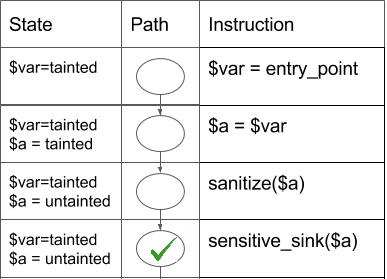
\includegraphics[width=.5\linewidth]{right.png}
		\caption{figure}{A figure}
		\label{fig:right}
	\end{minipage}%
	\begin{minipage}{.5\textwidth}
		\centering
		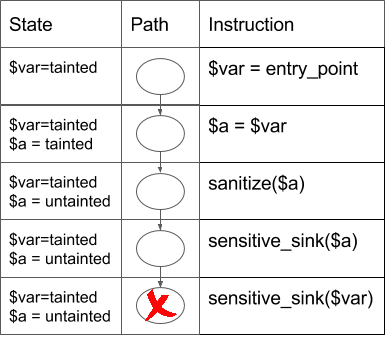
\includegraphics[width=.5\linewidth]{wrong.png}
		\caption{figure}{Another figure}
		\label{fig:wrong}
	\end{minipage}
\end{figure}

\section{Related Work}

%
% Bibliography
%
\bibliographystyle{plain}
\addcontentsline{toc}{section}{References}
\bibliography{references.bib}

\end{document}
